\section{nmap}
\label{tool:nmap}
\subsection*{Introduction}
\subsection{Nmap helper}
\href{https://github.com/leonjza/awesome-nmap-grep}{awesome-nmap-grep}

\subsubsection*{Port Status}
\begin{itemize}
    \item \textbf{open}: This indicates that the connection to the scanned port has been established. These connections can be TCP connections, UDP datagrams as well as SCTP associations.
    \item \textbf{closed}: When the port is shown as closed, the TCP protocol indicates that the packet we received back contains an RST flag. This scanning method can also be used to determine if our target is alive or not.
    \item \textbf{filtered}: Nmap cannot correctly identify whether the scanned port is open or closed because either no response is returned from the target for the port or we get an error code from the target.
    \item \textbf{unfiltered}: This state of a port only occurs during the TCP-ACK scan and means that the port is accessible, but it cannot be determined whether it is open or closed.
    \item \textbf{open|filtered}: If we do not get a response for a specific port, Nmap will set it to that state. This indicates that a firewall or packet filter may protect the port.
    \item \textbf{closed|filtered}: This state only occurs in the IP ID idle scans and indicates that it was impossible to determine if the scanned port is closed or filtered by a firewall.
\end{itemize}

\subsection*{Common usages}
\subsubsection*{Enumeration}
\label{tool:nmap:enumeration}

\begin{verbatim}
# will only calculate the IP to ping
nmap -sn -sL -n <domaine>/24

nmap -sn -n <domaine>/24

\end{verbatim}

\subsubsection*{Scripts}
\begin{verbatim}
# Default Scripts
nmap <target> -sC
# Specific Scripts Category
sudo nmap <target> --script <category>
# Defined Scripts
sudo nmap <target> --script <script-name>,<script-name>,...

nmap --script-help "afp-* and discovery"

cp ./http-shellshock.nse /usr/share/nmap/scripts/
sudo nmap --script-updatedb

SMB ENUM : nmap -p445 --script=smb-enum-shares.nse,smb-enum-users.nse 
NFS ENUM : nmap -p111 --script --script=nfs-ls,nfs-statfs,nfs-showmount
Banner grabing : --script=banner

smb-os-discovery.nse

\end{verbatim}


\subsection*{Options}

\begin{itemize}
    \item \verb+--reason+
    \item \verb+--packet-trace+
    \item \verb+-n+: no DNS
    \item \verb+--top-ports=NUM+
    \item \verb+-p-+
    \item \verb+-pNUM,NUM,...+
    \item \verb+-F+: equals \verb+--top-ports=100+
    \item \verb+-sC+: equals \verb+--script default+
\end{itemize}


\subsubsection*{Discovery}

\begin{itemize}
    \item \verb+--disable-arp-ping+
    \item \verb+--packet-trace+
\end{itemize}

\subsubsection*{Scan}



\begin{itemize}
    \item \verb++
\end{itemize}

\subsubsection*{Port}

\begin{itemize}
    \item \verb++
\end{itemize}

\subsubsection*{Script}

\begin{itemize}
    \item auth : Determination of authentication credentials.
    \item broadcast: Scripts, which are used for host discovery by broadcasting and the discovered hosts, can be automatically added to the remaining scans.
    \item brute: Executes scripts that try to log in to the respective service by brute-forcing with credentials.
    \item default: Default scripts executed by using the -sC option.
    \item discovery: Evaluation of accessible services.
    \item dos: These scripts are used to check services for denial of service vulnerabilities and are used less as it harms the services.
    \item exploit: This category of scripts tries to exploit known vulnerabilities for the scanned port.
    \item external: Scripts that use external services for further processing.
    \item fuzzer: This uses scripts to identify vulnerabilities and unexpected packet handling by sending different fields, which can take much time.
    \item intrusive: Intrusive scripts that could negatively affect the target system.
    \item malware: Checks if some malware infects the target system.
    \item safe: Defensive scripts that do not perform intrusive and destructive access.
    \item version: Extension for service detection.
    \item vuln: Identification of specific vulnerabilities.
\end{itemize}




\subsubsection*{Performance}
Options which take <time> are in seconds, or append 'ms' (milliseconds),
  's' (seconds), 'm' (minutes), or 'h' (hours) to the value (e.g. 30m).
\begin{itemize}
    \item \verb+-T<0-5>+: Set timing template (higher is faster)
    \item \verb+--min-hostgroup/max-hostgroup <size>+: Parallel host scan group sizes
    \item \verb+--min-parallelism/max-parallelism <numprobes>+: Probe parallelization
    \item \verb+--min-rtt-timeout/max-rtt-timeout/initial-rtt-timeout <time>+: Specifies probe round trip time.
    \item \verb+--max-retries <tries>+: Caps number of port scan probe retransmissions.
    \item \verb+--host-timeout <time>+: Give up on target after this long
    \item \verb+--scan-delay/--max-scan-delay <time>+: Adjust delay between probes
    \item \verb+--min-rate <number>+: Send packets no slower than <number> per second
    \item \verb+--max-rate <number>+: Send packets no faster than <number> per second
\end{itemize}

\begin{figure}
  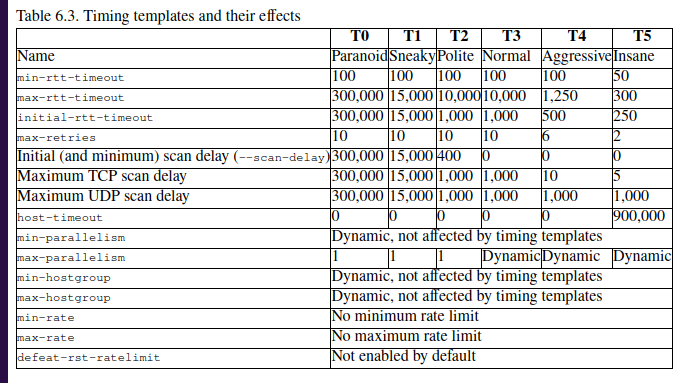
\includegraphics[width=\linewidth]{tools/all/images/nmap_timing_templates.png}
  \caption{nmap timing templates}
  \label{fig:nmap_timing_templates}
\end{figure}


\subsubsection*{Firewall and IDS/IPS evasion}
\begin{itemize}
    \item \verb+-g, --source-port <number>+: source port manipulation use 53
    that is usually enabled.
    \item \verb+-f, --mtu <val>+: fragment packets multiple of 16
    \item \verb+-D+ decoy \verb+IP_1:...:IP_n+ or \verb+RND:<number>+
\end{itemize}


\subsubsection*{Output}
\begin{itemize}
\item \verb+-oA <FILE>+: all
\item \verb+-oN <FILE>+: normal
\item \verb+-oG <FILE>+: grepable
\item \verb+-oX <FILE>+: xml
\item \verb+-v+: Increase verbosity level (use -vv or more for greater effect)
\item \verb+-d+: Increase debugging level (use -dd or more for greater effect)
\item \verb+--reason+: Display the reason a port is in a particular state
\item \verb+--stats-every=5s+

\end{itemize}

\subsection*{Scripts}
\subsubsection*{Enum Users (Kerberos pre-auth}
\label{tool:nmap:user-enum}
\begin{verbatim}
--script krb5-enum-users --script-args \
        krb5-enum-users.realm='DOMAIN.NAME',\
        userdb=USER_FILE_PATH
\end{verbatim}

\subsubsection*{SMB}
\label{tool:nmap:smb}


\subsection*{links}
\url{https://nmap.org/book/toc.html}
